%%% Local Variables: 
%%% mode: latex
%%% TeX-master: t
%%% End: 

\documentclass{article}
\usepackage[latin1]{inputenc}
\usepackage{graphicx}
\usepackage{color}
\usepackage{url}

% he insertado los comentarios y correcciones de pedro y lo añado como autor

\title{Experimentación con algoritmos distribuidos usando herramientas libres y gratuitas}

\author{Dr. Juan Julián Merelo Guervós, Dra. Maribel García Arenas, Pedro A. Castillo Valdivieso (Universidad de Granada)\\
Dr. Rodolfo García Bermúdez (Universidad de Holguín) y \\
MSc. José Albert Cruz Almaguer (Universidad de las Ciencias Informáticas, La Habana)
}

\begin{document}

\maketitle

\begin{abstract}
En un entorno de restricción de costes para grandes instalaciones
computacionales, acompañado de la existencia de herramientas en la nube
y ordenadores de sobremesa de altas capacidades, la experimentación
con algoritmos distribuidos se puede hacer fácilmente combinando ambas
cosas. En este trabajo se presenta una metodología de experimentación
con algoritmos genéticos distribuidos usando servicios de
almacenamiento en la nube tales como Dropbox (o alternativas libres
auto-instalables) y aplicaciones para gestión de máquinas virtuales
tales como VirtualBox. Usando el almacenamiento en la nube como un
sistema de intercambio de soluciones entre los diferentes nodos, se
tratará de probar la aplicabilidad de esta metodología así como probar
las capacidades de estos nuevos algoritmos evolutivos distribuidos. 
\end{abstract}

\section{Introducción}

La computación paralela no necesita ser complicada y prever escenarios
complejos o grandes variaciones de estructura de los programas
secuenciales. La mayor parte de los ordenadores actuales pueden
trabajar cómodamente con muchos procesos ejecutándose simultáneamente
y poseen sistemas de almacenamiento rápido que pueden usarse para
intercambiar información. Implementar un algoritmo que funcione de
forma concurrente es, por lo tanto, tan simple como ejecutar varios
procesos simultáneamente y que intercambien información a través de un
directorio especialmente designado para ello. La eficiencia de la
implementación no tiene por qué ser grande (y dependerá sobre todo del
tipo de procesador, del número de núcleos que posea y de la velocidad
y eficiencia del sistema de ficheros) pero, sin embargo, la
simplicidad en la programación es tal que puede compensar la menor
ganancia en velocidad obtenida de esta forma. 
% - pedro -
Además, añadir nuevos nodos de computación al sistema paralelo distribuido 
resultará extremadamente simple.

Simultáneamente, está cada vez más vigente el uso de infraestructuras
{\em nube} que permiten usar desde un ordenador conectado a la red
diferentes recursos tales como CPUs virtuales o discos duros
virtuales. El hecho de que sean {\em virtuales} implica que aparezcan,
desde el punto de vista del interfaz de programación, como si se
tratara de otras infraestructuras disponibles desde el sistema
operativo. En la práctica, podemos usar un disco duro remoto situado
en la nube como si se tratara de un disco duro local. De esta forma,
también simple y transparente al programador podemos paralelizar un
algoritmo, simplemente usando una infraestructura de almacenamiento
virtual. A la vez, en algunos casos estas infraestructuras son
gratuitas, bien por el hecho de que formen parte de la misma
organización (discos conectados a la red, NAS o bien infraestructuras
creadas con OpenStack u OpenNebula) o bien porque se trate de
productos comerciales que poseen una versión gratuita, como se trata
de Dropbox, Ubuntu One u otros. 

En este trabajo mostramos la primera aproximación al uso de
infraestructuras virtuales para la creación de experimentos de
computación distribuida de forma gratuita. Estos experimentos los
aplicaremos a un tipo de algoritmo denominado algoritmo genético. 
% - pedro - ¿no deberíamos referenciar los trabajos del dropbox anteriores?

%AUTORES: M.G. Arenas, J.J. Merelo, A.M. Mora, P.A. Castillo, G. Romero, J.L.J. Laredo
%TÍTULO: Assessing speed-ups in commodity cloud storage services for distributed evolutionary algorithms TIPO DE PARTICIPACIÓN: Oral
%CONGRESO: 2011 IEEE Congress on Evolutionary Computation
%PUBLICACIÓN: isbn 978-1-4244-7833-0/11 pp.304-311. 2011

%AUTORES: M. García-Arenas, J.J. Merelo, Pedro A. Castillo, J.L.J. Laredo, G. Romero and Antonio Miguel Mora 
%TÍTULO: Using free cloud storage services for distributed evolutionary algorithms
%CONGRESO: 13th Annual Genetic and Evolutionary Computation Conference, GECCO 2011
%PUBLICACIÓN: Proceedings, Dublin, Ireland, July 12-16, 2011. Natalio Krasnogor and Pier Luca Lanzi, Editors. ACM. pages 1603-1610. isbn 978-1-4503-0557-0. 2011

%AUTORES: Maribel Garcia-Arenas, Pedro Castillo Valdivieso, Gustavo Romero Lopez and Juan Julian Merelo Guervos 
%TÍTULO: Cloud-based Evolutionary Parallel Computation using low cost storage services
%PUBLICACIÓN: IEEE First International Symposium on Network Cloud Computing and Applications. isbn: 978-0-7695-4550- 9/11. pp.56-61. 2011. DOI 10.1109/NCCA.2011.16. 2011


Los algoritmos genéticos \cite{guervos2010informatica} son métodos de búsqueda y optimización
inspirados en la selección natural propuesta por
Darwin. Un algoritmo evolutivo codifica un problema en unas
estructuras de datos generalmente denominadas {\em cromosomas} y que
son una representación informática de los parámetros necesarios para
resolverlo; por ejemplo, resolver el recorrido del viajante implicaría
codificar en un {\em cromosoma} la lista de las ciudades a visitar; un
problema que tuviera varios números reales como parámetros usaría una
representación binaria con una precisión determinada de tales
parámetros, esta representación binaria es la que se usa en muchos
problemas numéricos y será la que usemos aquí por simple
conveniencia. 

Un algoritmo genético necesita una función de adecuación o {\em
  fitness} que nos permita evaluar lo que se acerca cada {\em
  cromosoma} a la solución. Esta función permite comparar diferentes
cromosomas y en principio y para simplificar, podemos pensar que es un
solo número real, aunque puede ser un vector o incluso tratarse de una
evaluación por parte de un usuario. La cuestión es que esta función
nos debe permitir evaluar qué cromosoma codifica una mejor solución al
problema que tratamos de resolver.

Una vez establecidos estos dos componentes del algoritmo, un algoritmo
evolutivo procede de la forma siguiente\begin{enumerate}
\item Se genera una población de cromosomas de tamaño $P$ y se evalúa
\item Mientras no se cumpla una condición de terminación (número de
  iteraciones, acercamiento a la solución o bien haber encontrado la
  solución, por ejemplo)\begin{enumerate}
  \item Escoger (de diferentes formas posibles) qué miembros de la
    población van a reproducirse, es decir, ser transformados para
    pasar a la siguiente iteración (denominada habitualmente {\em
      generación}, por el símil con la evolución natural.
  \item Cambiar una parte del cromosoma ({\em mutar}) o combinar dos
    soluciones ({\em entrecruzamiento}) para dar una nueva generación
    de cromosomas.
  \item Evaluar los nuevos individuos. Insertar esta nueva población
    en la población antigua, eliminando (en general) los peores. 
  \end{enumerate}
\end{enumerate}

Desde el punto de vista de este trabajo, lo interesante de los
algoritmos evolutivos es que se prestan a una fácil paralelización:
simplemente dividiendo la población en varias {\em islas} y creando  % - pedro -  una cita aquí
algún mecanismo de intercambio de individuos entre las islas.

Esto es precisamente lo que vamos a hacer en este trabajo. Usaremos un
algoritmo genético  que, dividido en varias {\em islas}, intercambiará
información a través de un directorio compartido. Ese directorio
compartido puede estar en un servicio tal como Dropbox, pero en este
caso no haremos experimentos relacionados con esto.   % - pedro - esta frase me resulta ¿como contradictoria? da la impresión de que va a ser que sí, pero tras la coma, resulta ser que no!
Trabajaremos además usando un sistema de fuentes abiertas en el que tanto el código
como la experimentación como este mismo trabajo están a disposición
de la comunidad científica desde el momento de su creación.  % - pedro -  decir dónde estarán para bajarlo

Con este trabajo tratamos de demostrar que, usando un mecanismo de
intercambio a través de almacenamiento, se pueden conseguir mejoras de velocidad incluso en un
sólo ordenador; para ello probaremos desde uno a cuatro
procesos. Además, haremos ciertos experimentos preliminares que nos
permitan saber qué políticas de migración son las más adecuadas.

El resto del trabajo se organiza como sigue: a continuación exponemos
los resultados más sobresalientes en este área. Posteriormente
explicamos el algoritmo y la metodología de experimentación
usada en la Sección \ref{sec:imp}. Finalmente expondremos los resultados obtenidos y las
conclusiones derivadas de los mismos para terminar con algunas notas
de trabajo futuro en la Sección \ref{sec:res}. 


\section{Estado del arte}

Los principales resultados en este área son de los mismos autores
\cite{DBLP:conf/cec/ArenasGMCRL11,DBLP:conf/gecco/ArenasGCLRM11,mericloud}. En   % - pedro -  aquí sí se citan los trabajos propios anteriores
estos trabajos se usó un algoritmo evolutivo implementado en Java para
probar diferentes sistemas gratuitos de almacenamiento en nube tales
como Dropbox u otros. Como principal resultado se obtuvo el hecho de
que se conseguían escalados interesantes, pero sólo con unas pocas
máquinas. Además, el retraso en la propagación de los resultados de
unas máquinas a otras implicaba que el problema de optimización debía
de ser de cierto tamaño para que los resultados fueran
significativos. El principal problema era que, debido a este retraso
en la propagación, la migración introducía también un retraso en la
ejecución del algoritm para que esta fuera capaz de propagarse. 

En este trabajo principalmente tratamos de reproducir los resultados
obtenidos en el mismo con otro tipo de implementación y, además,  % - pedro -  indicar qué tipo de implementación
usando otra implemenatción diferente que tiene como principal
diferencia el hecho de no tener en cuenta si el algoritmo se está
ejecutando secuencialmente o conjuntamente con otros nodos. Veremos en
la sección siguiente estos detalles de implementación. 

\section{Detalles de implementación y experimentos}
\label{sec:imp}

Para hacer los experimentos se ha usado la librería {\tt
  Algorithm::Evolutionary::Simple}, un módulo en Perl realizado por
uno de los autores que permite crear un algoritmo genético rápidamente
y en pocos pasos. La librería en Perl está optimizada para trabajar
rápidamente \cite{DBLP:conf/iwann/MereloRACML11} a pesar de tratarse
de un lenguaje interpretado como el Perl. Este lenguaje, por otro lado, resulta
un lenguaje bastante adecuado para trabajar, en general, con
algoritmos evolutivos teniendo una variedad de herramientas, algunas
de las cuales han sido creadas por los autores de este trabajo
\cite{perl-ea}.

Para hacer los experimentos se ha buscado un problema que represente
cierto reto para un algoritmo genético y cuya evaluación también
requiera cierto tiempo, de forma que el algoritmo necesite un número
de evaluaciones alto que pueda mejorarse a base de la
paralelización. Por eso la función elegida ha sido P-Peaks
\cite{alba2002comparing}. En esta función se general aleatoriamente un conjunto
de $p$ cadenas binarias de longitud $b$. P-Peaks devuelve la distancia
a la cadena {\em más cercana}, es decir, el mínimo de las distancias
medida a todas las cadenas. La función resulta {\em pesada} porque hay
que medir distancias a un número determinado de cadenas y resulta
complicada para un algoritmo evolutivo al tener un número alto de
máximos globales (correspondientes a cada una de las cadenas que se
han generado). La implementación de esta función es también libre,
está escrita en Perl y forma parte del módulo {\tt
  Algorithm::Evolutionary} denominándose {\tt
  Algorithm::Evolutionary::Fitness::P\_Peaks}. 
% - pedro - pon una nota a pie indicando que está en el CPAN (para que lo bajen)

Los parámetros base usados en el algoritmo evolutivo se muestran en la
tabla \ref{tab:params}. En general, son los valores por omisión de la
librería.  
%
\begin{table}[t!]
\centering 
\caption{Valores de los parámetros del algoritmo genético y de la
  función P-Peaks usada. \label{tab:params}}
\begin{tabular}{lc}
\hline
Parámetro & Valor \\
\hline \\
Selección & Rueda de ruleta \\
Mutación & 1-bit \\
Entrecruzamiento & 2 puntos \\
$P$ (número de picos)  & 256 \\
$b$ (bits del cromosoma)   & 512 \\ 
Población base & 1024 \\
\hline
\end{tabular}
\end{table}
%
Sin embargo, como se ha comentado, $P$ y $b$ han sido elegidos para
hacer el trabajo suficientemente difícil como para que cada ejecución
del algoritmo dure un tiempo considerable. Por otro lado, tratándose
de un problema difícil, se ha escogido un tamaño grande de población
para que el algoritmo sea capaz de encontrar la solución; con tamaños
más pequeños de población (o subdivisiones del tamaño) se vio que en
muchos casos el algoritmo se quedaba estancado y era incapaz de
encontrar la solución.

Para probar las prestaciones en paralelo del algoritmo se dividió la
población entre dos y entre cuatro y se probó con un número igual de
procesos. Los procesos se lanzaban desde un guión de línea de órdenes  % - pedro -  "guión" ???
de Linux de forma que eran más o menos simultáneos. Había un proceso
{\em principal} y otros {\em secundarios}; la principal diferencia es
que este proceso {\em principal} decide cuando comienza y termina cada
algoritmo y se usa también para medir la duración de los mismos. Esto
puede significar que, si la solución se encuentra por primera vez en
alguno de los procesos secundarios, el programa puede continuar
durante un tiempo adicional; sin embargo, no suele demorarse mucho
dado que se intercambian cromosomas entre unos procesos y otros. El
hacerlo así, además, evita que hagan falta mecanismos adicionales de
comunicación del final que tengan que propagarse y simplifica la
programación que, en realidad, es exactamente la misma para el
programa secuencial y el paralelo. El tiempo de ejecución se mide
simplemente a través de la diferencia en segundos entre el tiempo de
creación de dos ficheros que se crear, precisamente, al comenzar y
terminar este programa. 

Para la versión paralela hace falta una {\em política de
  migración}. En nuestro caso se ha elegido depositar un cromosoma      % - pedro -   "depositar" me suena raro, pero no se me ocurre otro verbo...
aleatorio elegido entre el 50\% con más fitness y tomar, a la vez, uno
aleatorio del directorio en el que lo han depositado el resto. El
elegir uno aleatorio entre los mejores coincide con la política que
suele obtener mejores resultados en modelos isla, según hemos podido
establecer en el pasado \cite{jj:2008:PPSN}. De hecho, algunas pruebas
hechas depositando el mejor en cada generación ha dado peores
resultados, provocando que en la mayor parte de los casos no termine
el algoritmo. La estrategia aleatoria, aparte de rápida (no necesita
ordenar ni hacer ninguna otra operación) tiene la ventaja de la
estrategia de depósito de chromosomas: no necesita tampoco llevar a
cabo ningún cambio en el código para el caso paralelo.

Tanto el código como el resultado de los experimentos (que
analizaremos en la siguiente sección) están disponibles de forma
abierta en la siguiente dirección:
\url{https://code.launchpad.net/\~jjmerelo/simplea/trunk}. El objetivo
es que la comunidad científica se beneficie de esta ciencia abierta no
sólo en los resultados, sino también en los datos que podrán ser, en
caso de desearlo, analizados de forma independiente. 

\section{Resultados, conclusiones y trabajo futuro}
\label{sec:res}

Los experimentos se ejecutaron 10 veces. En todos los casos se
encontró la solución, salvo en el caso en el que se hizo con cuatro
nodos, en el que acabó sólo en 6 ocasiones. En todo caso, los
resultados se muestran sobre los que efectivamente terminaron.

El primer resultado es que efectivamente, a pesar de ejecutarse en un
sólo ordenador y cargar la tabla de procesos del mismo, se consigue
una mejora en la velocidad con el número de {\em nodos}. Esto se
muestra en las Figuras \ref{fig:sm} y \ref{fig:toshiba}; en el primer
caso los tiempos han sido tomados en un ordenador AMD con séxtuple
núcleo ejecutando Ubuntu 12.04; en el segundo es un portátil Toshiba
Portegé ejecutando el mismo sistema operativo y con un Intel i5 de
procesador; en este caso el disco duro es un SSD lo que lo hace,
teóricamente, más rápido que en el primer caso.

% - pedro -   no están las imágenes en el directorio (para compilar el paper)

\begin{figure*}[!htb]
\centering
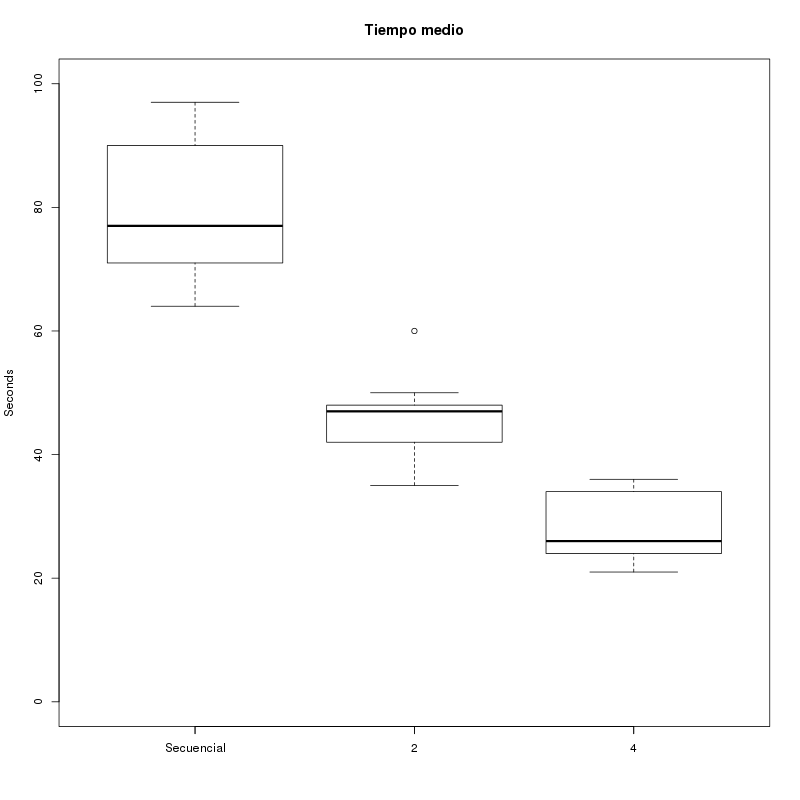
\includegraphics[scale=0.45]{tiempos.png}
\caption{Boxplot del tiempo medio (en segundos) necesario para
  terminar el algoritmo usando un programa secuencial y dos y cuatro
  procesos simultáneos.  Los tiempos han sido tomados en un ordenador
  de sobremesa. \label{fig:sm}}
\end{figure*} 
%
\begin{figure*}[!htb]
\centering
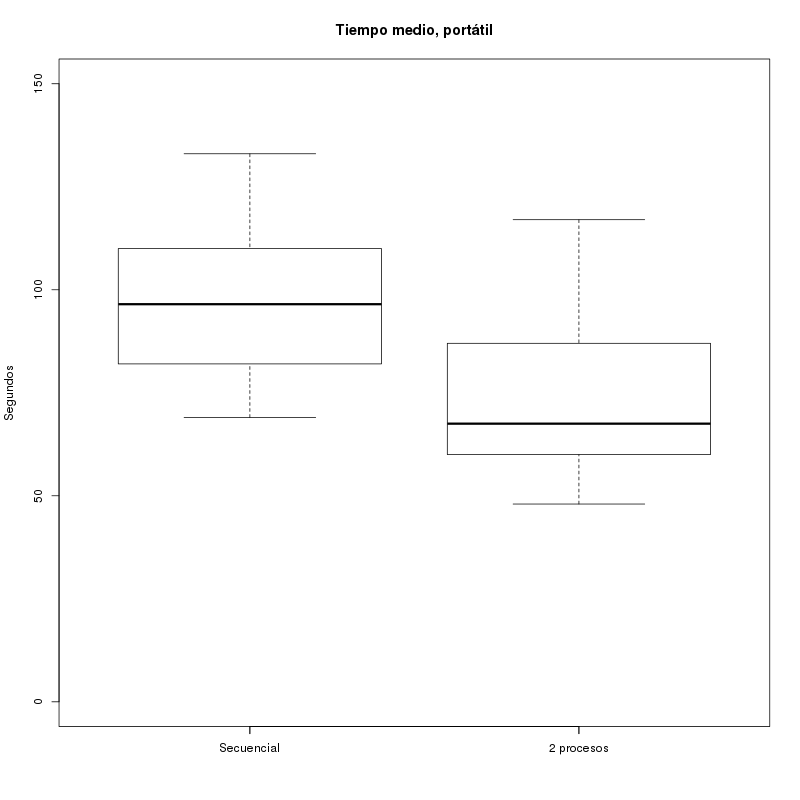
\includegraphics[scale=0.45]{tiempos-toshiba.png}
\caption{Boxplot del tiempo medio (en segundos) necesario para
  terminar el algoritmo usando un programa secuencial y dos 
  procesos simultáneos en un ordenador portátil.  \label{fig:toshiba}}
\end{figure*} 
%
\begin{figure*}[!htb]
\centering
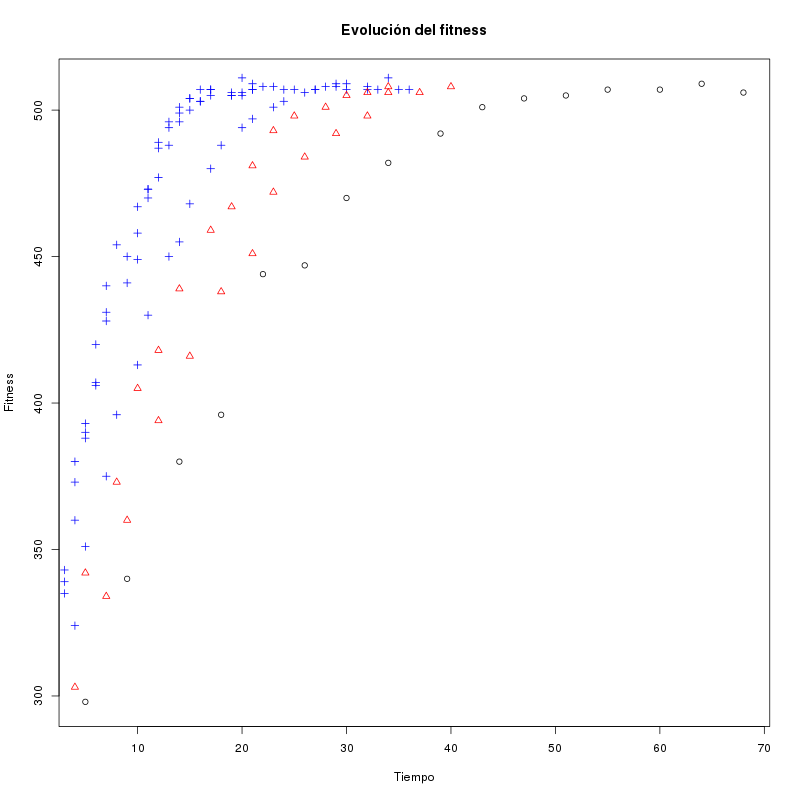
\includegraphics[scale=0.45]{evolucion-fitness.png}
\caption{Evolución del fitness de una instancia de cada uno de los
  tres experimentos; los círculos indican el experimento con un solo
  proceso, los triángulos con dos y las cruces con 4 procesos. El
  tiempo en el eje de abscisas es el tiempo real; el fitness máximo es
  512.  \label{fig:fit}}
\end{figure*} 

Como se puede ver en ambas gráficas, el añadir nodos consigue rebajar
el tiempo necesario para hallar la solución. De hecho, parte de esta
mejora se debe al hecho de que se usen menos individuos en la
población; pero una parte también se debe a que se están evaluando
simultáneamente más individuos. De hecho, la mejora para cuatro nodos
es de un 70\% en la velocidad en el primer caso, mientras que la
mejora para dos nodos es de un 40\% en el segundo caso, algo mejor en
el primer caso. Esto, en parte, puede deberse al hecho de que
realmente no nos preocupamos de cuando halla la solución cualquier
nodo, sino sólo cuando la halla uno de ellos; pero en parte también a
que se nota la carga del sistema al ejecutar varios procesos
simultáneamente, sea en la CPU sea en entrada salida.   % - pedro -   cambiar la redacción de esta frase (no entiendo a partir de la coma
De hecho, en el
primer caso las tres diferencias son significativas usando el test no
paramétrico de Wilcoxon, mientras que en el segundo caso la diferencia
no es significativa. Esto puede significar que la mayor velocidad del
disco duro haga que la diferencia entre uno y otro sea menor al
dedicar menos tiempo al escribir en disco; esto podría indicar que uno
de los factores que influyen en el tiempo es el tiempo empleado en
leer del sistema de ficheros. Habrá que evaluar mediante un profiler  % - pedro -  comentar esto en los trabajos futuros
este tipo de hipótesis para probar si es cierta o no, aunque una
evaluación preliminar indica que el tiempo invertido en leer y
escribir del disco duro es tres órdenes de magnitud inferior al tiempo
total del programa. 

Por otro lado, en el primer caso se puede ver en la figura
\ref{fig:fit} la evolución procede de forma bien diferente dependiendo
del número de procesos. En este caso lo que se traza para cada número
de procesos es el tiempo de creación del fichero co el individuo que
se está migrando tomado directamente del sistema de ficheros; el
tiempo tiene resolución de segundos; esto es una ventaja adicional de
usar este sistema, que te permite ver la evolución, con el tiempo, del
fitness. Si recordamos que en realidad el que se graba es un individuo
aleatorio entre los 50\% mejores, vemos que, en todo caso y para un
tiempo determinado, por ejemplo 10 segundos, cuando hay 4 nodos se ha
avanzado mucho más que cuando se usan dos o un solo nodo; esto prueba
que el algoritmo evolutivo se puede paralelizar usando este simple
mecanismo que es, también, extensible a sistemas que permitan
almacenamiento transparente en la nube como Dropbox, tal como
queríamos probar.

Adicionalmente hemos hecho alguna prueba con directorios compartidos a
través de Dropbox y alojados en diferentes máquinas virtuales dentro
del mismo ordenador. 
Esto presenta una serie de retos, el principal   % - pedro -   la segunda parte de esta frase no la entiendo
que la velocidad de tales máquinas virtuales va a ser muy diferente y
continuando con el problema del retraso en la aparición de los
ficheros individuales en el resto de los nodos. 
Sin embargo, algunas pruebas iniciales (que se pueden ver en el repositorio de código y
datos indicados) indican que, aunque se consiguen ciertas mejoras al
añadir un nuevo nodo, no está claro que sean significativas, por lo
que hay que avanzar haciendo experimentos en este sentido, probando
con diferentes configuraciones, máquinas virtuales y parametrización
de las mismas. Esto es algo que se propone como trabajo futuro.


% - pedro -  ¿no hay sección de conclusiones y trabajos futuros como tal?


\section{Agradecimientos}
Este trabajo está apoyado por los proyectos 
TIN2011-28627-C04-02 del Ministerio español de Ciencia y
Competitividad y por el P08-TIC-03903 del gobierno regional andaluz,
así como el proyecto 83 (CANUBE) concedido por el CEI-BioTIC UGR
(\url{http://biotic.ugr.es}). 

\bibliographystyle{plain}
\bibliography{dr,geneura}

\end{document}
